%%%%%%%%%%%%%%%%%%%%%%%%%%%%%%%%%%%%%%%%%%%%%%%%%%%%%%%%%%%
\subsection{Mueller Matrices}
%%%%%%%%%%%%%%%%%%%%%%%%%%%%%%%%%%%%%%%%%%%%%%%%%%%%%%%%%%%
Interactions with materials that can create depolarization and model partially polarized input and outputs cannot be handled by Jones calculus.  For these problems, Mueller Matrices are used to model the polarization of light with varying degrees of polarization as it interacts with a material.  These interactions are modeled with equation [CHECK add system diagram here with boxes] and shown in Figure.
\begin{align}
    \mathbf{S}_{out} = \mathbf{M}\mathbf{S}_{in}
\end{align}
%
When EM waves interact with optically active materials, their state of polarization may change.  The characteristics of a material which changes the amplitude or phase of the $x$ or $y$ component for an incident EM wave, i.e. the  polarization, is defined by its Mueller matrix.  Mueller matrices determine how input Stokes' vectors change upon interaction with a material. They are defined as
%
\begin{align}
    \mathbf{M} =
    \begin{bmatrix}
        m_{00} & m_{01} & m_{02} & m_{03} \\
        m_{10} & m_{11} & m_{12} & m_{13} \\
        m_{20} & m_{21} & m_{22} & m_{23} \\
        m_{30} & m_{31} & m_{32} & m_{33}
    \end{bmatrix}
\end{align}
%
and describe the diattenuation, depolarization, and retardance of a materials' polarization response to an input EM beam.
%The general equation for polarization material interaction is
\begin{figure}
    \begin{center}
        \makebox[\textwidth]{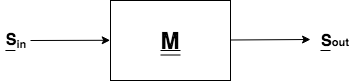
\includegraphics[scale=0.6]{/Sources/Background/Nature_of_Light/system_stokes.png}}
    \end{center}
    \caption{Stokes-Mueller System Diagram}
    \label{fig:polarization}
\end{figure}
%\begin{align}
%    \begin{bmatrix}
%        S_0 \\
%        S_1 \\
%        S_2 \\
%        S_3
%    \end{bmatrix}
%        m_{00} & m_{01} & m_{02} & m_{03} \\
%        m_{10} & m_{11} & m_{12} & m_{13} \\
%        m_{20} & m_{21} & m_{22} & m_{23} \\
%        m_{30} & m_{31} & m_{32} & m_{33}
%    \end{bmatrix}
%    \begin{bmatrix}
%        S_0^\prime \\
%        S_1^\prime \\
%        S_2^\prime \\
%        S_3\prime
%    \end{bmatrix}
%\end{align}

%[CHECK these get bolded]
\underline{Diattenuation} – the two attenuations of orthogonal polarization states \cite{chipman}

\underline{Retardance} – the phase difference between two orthogonal polarization states \cite{giakos}

\underline{Depolarization} – a process where polarized light becomes unpolarized \cite{giakos}

It has been shown that these parameters can be found by determining a sample's corresponding Mueller Matrix. The scalar parameters are mathematically defined as,
\begin{align}
    \mathbf{Diattenuation} = \frac{T_{max} - T_{min}}{T_{max} + T_{min}}
\end{align}
\begin{align}
    \mathbf{Retardance} = \delta = \frac{2\pi(n_1 - n_2)t}{\lambda}
\end{align}
\begin{align}
    \mathbf{Depolarization} = 1 - DOP
\end{align}
were $T_{max}$ and $T_{min}$ are the intensity transmittances through a polarizer, $n_1$, $n_2$ and $t$ are the refractive indices and thickness of a retarder \cite{chipman}.
[CHECK explain these equations or remove them]

For nondepolarizing materials, their MM can be converted into Jones matrices.   Examples of Mueller Matrices for common optical elements can be found in \cite{chipman}.  The general form of a linear polarizer with transmission axis at 0 degrees to the $x$ axis is
%
\begin{align}
    \mathbf{M} =
    \begin{bmatrix}
        q + r & q - r & 0 & 0 \\
        q-r & q+r & 0  & 0 \\
        0 & 0 & 2\sqrt{qr} & 0 \\
        0 & 0 & 0 & 2\sqrt{qr}
    \end{bmatrix}
\end{align}
%
where $q$ and $r$ are the attenuation coefficients for the $x$ and $y$ axis [TODO relate this to the later equation showing transmissiona and reflection].

%%%%%%%%%%%%%%%%%%%%%%%%%%%%%%%%%%%%%%%%%%%%%%%%%%%%%%
\subsubsection{Mueller Matrix Decomposition}
%%%%%%%%%%%%%%%%%%%%%%%%%%%%%%%%%%%%%%%%%%%%%%%%%%%%%%

The effects of diattenuation, depolarization and retardance can be found to be represented as subsets of the Muller matrix through its decomposition such that the result is
\begin{align}
    \mathbf{M} = m_{00}
    \begin{bmatrix}
        1 & \mathbf{D}^T \\
        \mathbf{P} & \mathbf{m}
    \end{bmatrix}
\end{align}
The derivation of the MM decomposition was made known by Lu and Chipman and is reproduced in \cite{polarizedlight}. $\mathbf{D}^T$ is the diattenutation vector that describes the amount of decrease in overall polarization for each set of orthogonal polarization states. The m matrix represents the retardance of a material.

$\mathbf{P}$ is the polarizance vector, and describes the amount of light that becomes polarized when unpolarized light is incident.  It is analogous to the effect of depolarization.  This vector can be measured by detecting the output Stokes vector of a material when unpolarized light is incident.  This effect is only evident in materials that create polarization.
